\documentclass[tikz]{standalone}

\usepackage[english]{babel}
\usepackage{amsmath}
\usepackage{amssymb}

\usepackage{tikz}
\usetikzlibrary{trees}
\begin{document}

\begin{center}
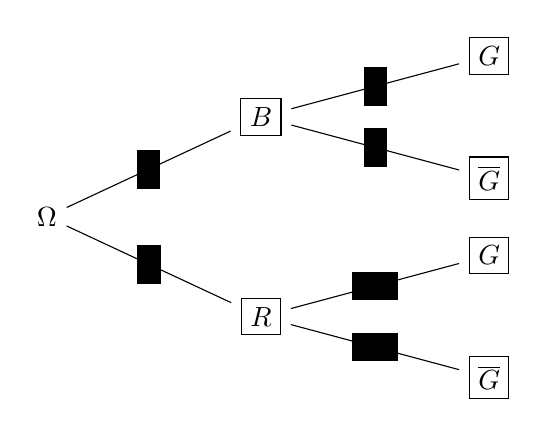
\begin{tikzpicture}[level distance=3cm] \tikzstyle{edge from parent}=[-,draw]
        \node {$\Omega$} [clockwise from=25, sibling angle=50]
            child {node {\fbox{$B$}} [clockwise from=15, sibling angle=30]
                child {node {\fbox{$G$}}
                edge from parent node[fill=black, inner sep=1pt] {$\frac{3}{5}$}}
                child {node {\fbox{$\overline{G}$}}
                edge from parent node[fill=black, inner sep=1pt] {$\frac{2}{5}$}}
            edge from parent node[fill=black, inner sep=1pt] {$\frac{1}{3}$}
            }
            child {node {\fbox{$R$}} [clockwise from=15, sibling angle=30]
                child {node {\fbox{$G$}}
                edge from parent node[fill=black, inner sep=1pt] {$0,3$}}
                child {node {\fbox{$\overline{G}$}}
                edge from parent node[fill=black, inner sep=1pt] {$0,7$}}
            edge from parent node[fill=black, inner sep=1pt] {$\frac{2}{3}$}
            };
    \end{tikzpicture}
\end{center}

\end{document}
